% ----------------------------------------------------------------------

\chapter{\textbf{A aprendizagem de máquina}} % Este comando é utilizado para criar capítulos

Desde os primórdios, a humanidade busca maneiras de aperfeiçoar suas técnicas e métodos para melhorar seus processos, seja com a descoberta do fogo para a preparação dos alimentos, a ferramentas para auxiliar o trabalho e qualidade de vida humana. A tecnologia é presente desde os primeiros resquícios de vida humana, sua notável evolução e a que proporcionou o conjunto tão completo de conhecimento e ciência, que hoje, proporciona uma melhoria essencial na qualidade de vida.\par
Em resumo, a informática e uso de diversas técnicas que proporcionam a automação da informação, desde uma calculadora manual, qual seus complexos sistemas de engrenagem proporcionam a utilização de funções matemáticas de forma simplificadas, a invenção do transistor, que proporcionou uma exponencial na evolução tecnológica humana. \par
Arbitrariamente, os computadores podem ser vistos como um livro aberto para a criatividade humana, são ınfimos as utilidades e aplicações, que dependem de grande parte da imaginação humana para a solução de problemas reais. \par
Como a maioria das criações, a aprendizagem de máquina nasce a partir da busca de uma solução para um problema real, mais especificamente, um simples jogo de damas. \cite{Samuel1959}, cientista da computação, pioneiro em aprendizado de máquina,
construiu um jogo de damas na qual seu adversário seria o computador, entretanto, o computador não conseguiu ganhar nenhuma das partidas, Arthur decide escrever um algoritmo no qual o computador analisa as partidas anteriores e aprendia as melhores estratégias dos jogos históricos, foram feitas diversas rodadas, e a partir de um certo momento, a máquina ganhava todas as rodadas. Com isso podemos iniciar o surgimento da aprendizagem de máquina, um problema aparentemente simples, que ao final se torna um novo ramo da computação.\par 
Segundo a definição clássica de \cite{Samuel1959}, O aprendizado de máquina é um campo de estudo no qual computadores têm a habilidade de aprender sem ter sido explicitamente programado para tal. \par
Diante da imensidão de aplicações, a aprendizagem de máquina torna-se uma aplicação de alta complexidade, incluindo a arquitetura distribuída, os principais problemas envolvem a dificuldade de escala dos projetos, gerando um alto custo. 


\section{O classificador} % Este comando é utilizado para criar capítulos
Neste tópico iremos abordar o classificador utilizado para a confecção da aplicação de machine learning utilizada como base de estudo, que no caso um dos classificadores clássicos, a floresta randômica. O algoritmo preditivo baseia-se na combinação de diversas árvores de decisão para chegar em um resultado único \cite{Breiman2001}. 
Uma simples analogia é de uma pessoa realizando a comparação de determinado computador, no caso a pessoa irá dispor a analisar o produto com seus concorrentes, comparando o preço,  funcionalidades, qualidade, desempenho, com base nessas informações históricas, determina qual será a melhor escolha a ser feita baseado nesses dados.




\begin{figure}[h!]
	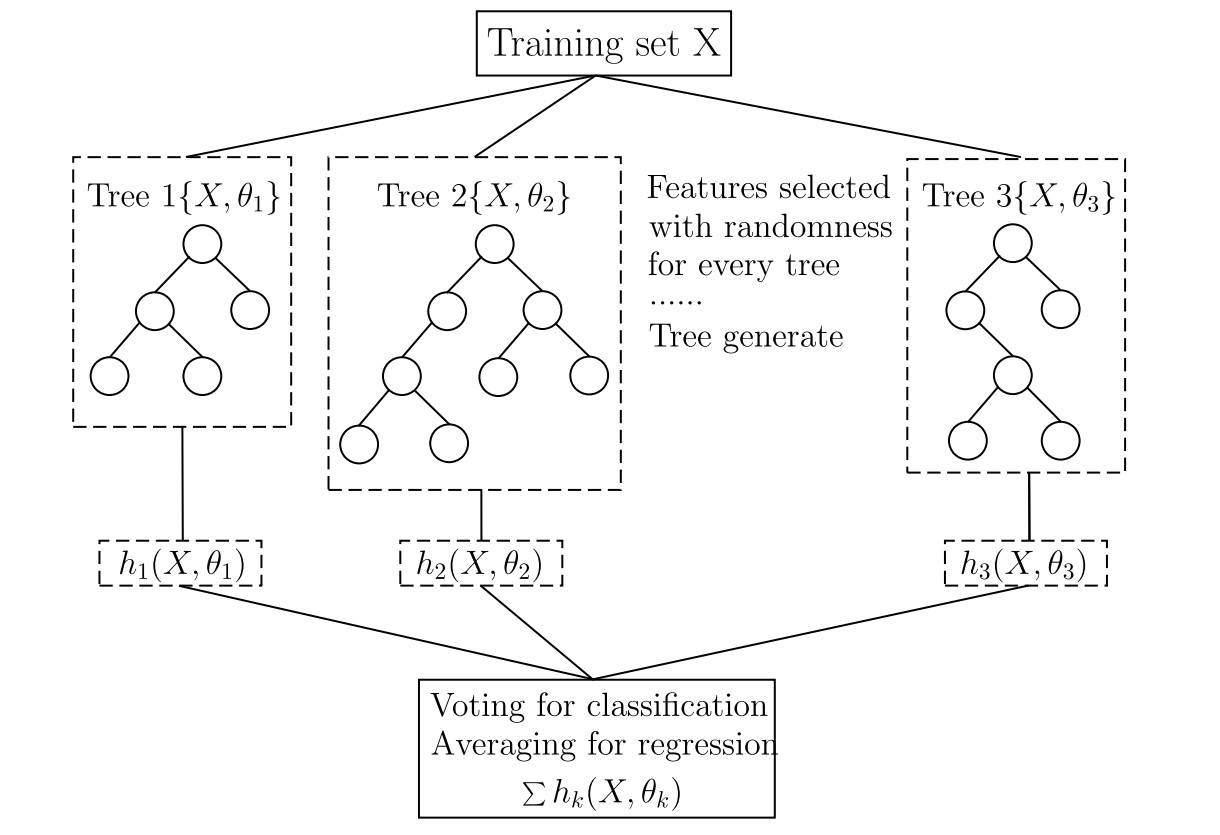
\includegraphics[width=\linewidth]{topics/chart.jpg}
	\caption{Fluxograma classificatório da florestas randômica, por \cite{Zhang2018}.}
	\label{fig:chartrandomforest}
\end{figure}



No caso do algoritmo, será feito uma análise dos dados, histórico para realização do treinamento do modelo, este modelo é composto de padrões matemáticos, ou seja, métricas gerais do comportamento histórico das informações. Com esses modelos gerados a partir de uma montanha de dados, será capaz o algoritmo realizar a predição de um novo dado, possibilitando a avaliação, por exemplo, de uma escolha boa ou ruim de determinado computador.